\documentclass[UTF8]{ctexart}

\usepackage{fancyhdr}
\usepackage{titlesec}
\usepackage{geometry}
\geometry{a4paper,left=2cm,right=2cm,bottom=2.5cm,top=2.5cm}
\usepackage{graphicx}
\usepackage{epstopdf}
\usepackage{listings}
\usepackage{indentfirst}
\usepackage{multirow}
\graphicspath{ {figure/} } 

\pagestyle{fancy}
\lhead{} 
\chead{\bfseries 光信息科学与技术实验} 
\rhead{} 
\lfoot{} 
\cfoot{\thepage}
\rfoot{} 
\renewcommand{\headrulewidth}{0.4pt} 
\renewcommand{\footrulewidth}{0.4pt}

\newcommand{\major}{计算机应用技术,精密仪器及机械}
\newcommand{\name}{杜沈达,王晨}
\newcommand{\stuid}{SA18168163,SA18168095}
\newcommand{\newdate}{\today}
\newcommand{\loc}{物理楼}
\newcommand{\course}{光信息科学与技术实验}
\newcommand{\grades}{}
\newcommand{\newtitle}{Nd:YAG激光放大器特性研究}

\makeatletter
\newcommand{\figcaption}{\def\@captype{figure}\caption}
\newcommand{\tabcaption}{\def\@captype{table}\caption}
\makeatother
\setlength{\parindent}{2.45em}

\begin{document}
\thispagestyle{empty}
	\begin{figure}[h]
		\begin{minipage}{0.6\linewidth}
			\includegraphics[width=\linewidth]{head.jpg}
		\end{minipage}
		\hfill
		\begin{minipage}{.4\linewidth}
			\raggedleft
			\begin{tabular*}{.8\linewidth}{ll}
				专业: & \underline\major   \\
				姓名: & \underline\name    \\
				学号: & \underline\stuid   \\
				日期: & \underline\newdate \\
				地点: & \underline\loc
			\end{tabular*}
		\end{minipage}
	\end{figure}
	
	\begin{table}[!htbp]
		\centering
		\begin{tabular*}{\linewidth}{llllll}
			课程名称: & \underline\course   & 
			实验名称: & \underline\newtitle & 
			成绩:     & \underline\grades \\
		\end{tabular*}
	\end{table}

\titleformat*{\section}{\large\bfseries}
\titleformat*{\subsection}{\normalsize\bfseries}
\titleformat*{\subsubsection}{\normalsize}

\section{实验目的}
\begin{enumerate}
	\item 了解固体激光器的自由振荡输出特性
	\item 了解固体激光器的应用
	\item 掌握固体激光器的光路调整
\end{enumerate}

\section{实验原理}
	\subsection{自由振荡激光输出特性}

自由振荡固体激光器输出激光脉冲特点是具有尖峰结构,即由许多振幅,脉宽和间隔作随机变化的尖峰脉冲组成,每个尖峰的宽度为$0.1~1\mu s$,间隔为数微秒,脉冲序列的时间长度大致等于闪光灯泵浦持续时间,这种现象称为激光的弛豫振荡。
	\begin{center}
		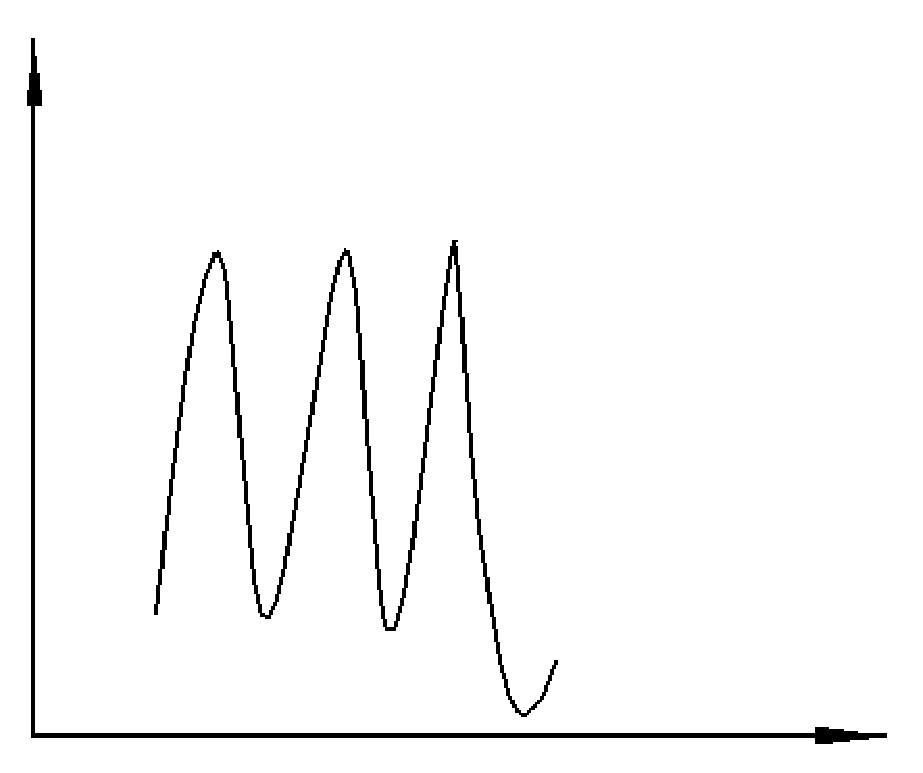
\includegraphics[width=12cm,height=6cm]{free.eps}
		\figcaption{激光自由振荡特性}\label{free.png}
	\end{center}
	
产生弛豫振荡的主要原因是:当激光器的工作物质被泵浦,上能级的粒子反转数超过阈值条件时,即产生激光振荡,使腔内光子数密度增加而发射激光。随着激光的发射,上能级粒子数大量被消耗,导致粒子反转数目降低,当低于阈值时又产生第二个脉冲,如此重复上述过程,知道泵浦停止才结束。可见每个尖峰脉冲都是在阈值附近产生的,因此脉冲的峰值功率水平较低,即增大泵浦能量也无助于峰值功率的提高,而只会使小尖峰的个数增加。
	
\subsection{自由振荡激光器的组成}
	
固体激光器是由三个主要部分组成的:工作物质,泵浦能源以及光学谐振腔。


\begin{tabular}{rl}
	工作物质:&掺钕钇铝石榴石($Nd^{3+}: YAG$) ($Y_{3}Al_{5}O_{12}$)\\
	泵浦能源:&由双椭圆聚光腔,泵浦脉冲氙灯,激光电源组成\\
	光学谐振腔:&两个相互平行的平面镜组成\\
\end{tabular}
\section{实验内容}
\begin{enumerate}
	\item 调整激光光路
	\item 测量自由振荡激光的输出特性
	\item 自由振荡及挂钩器的实际应用举例
\end{enumerate}
\subsection{实验步骤}
\begin{enumerate}
	\item 调整激光光路
	\begin{enumerate}
\item 先将准直光源$He-Ne$激光器对准$YAG$激光放大棒中心,固定不动。,如图2
		\begin{center}
			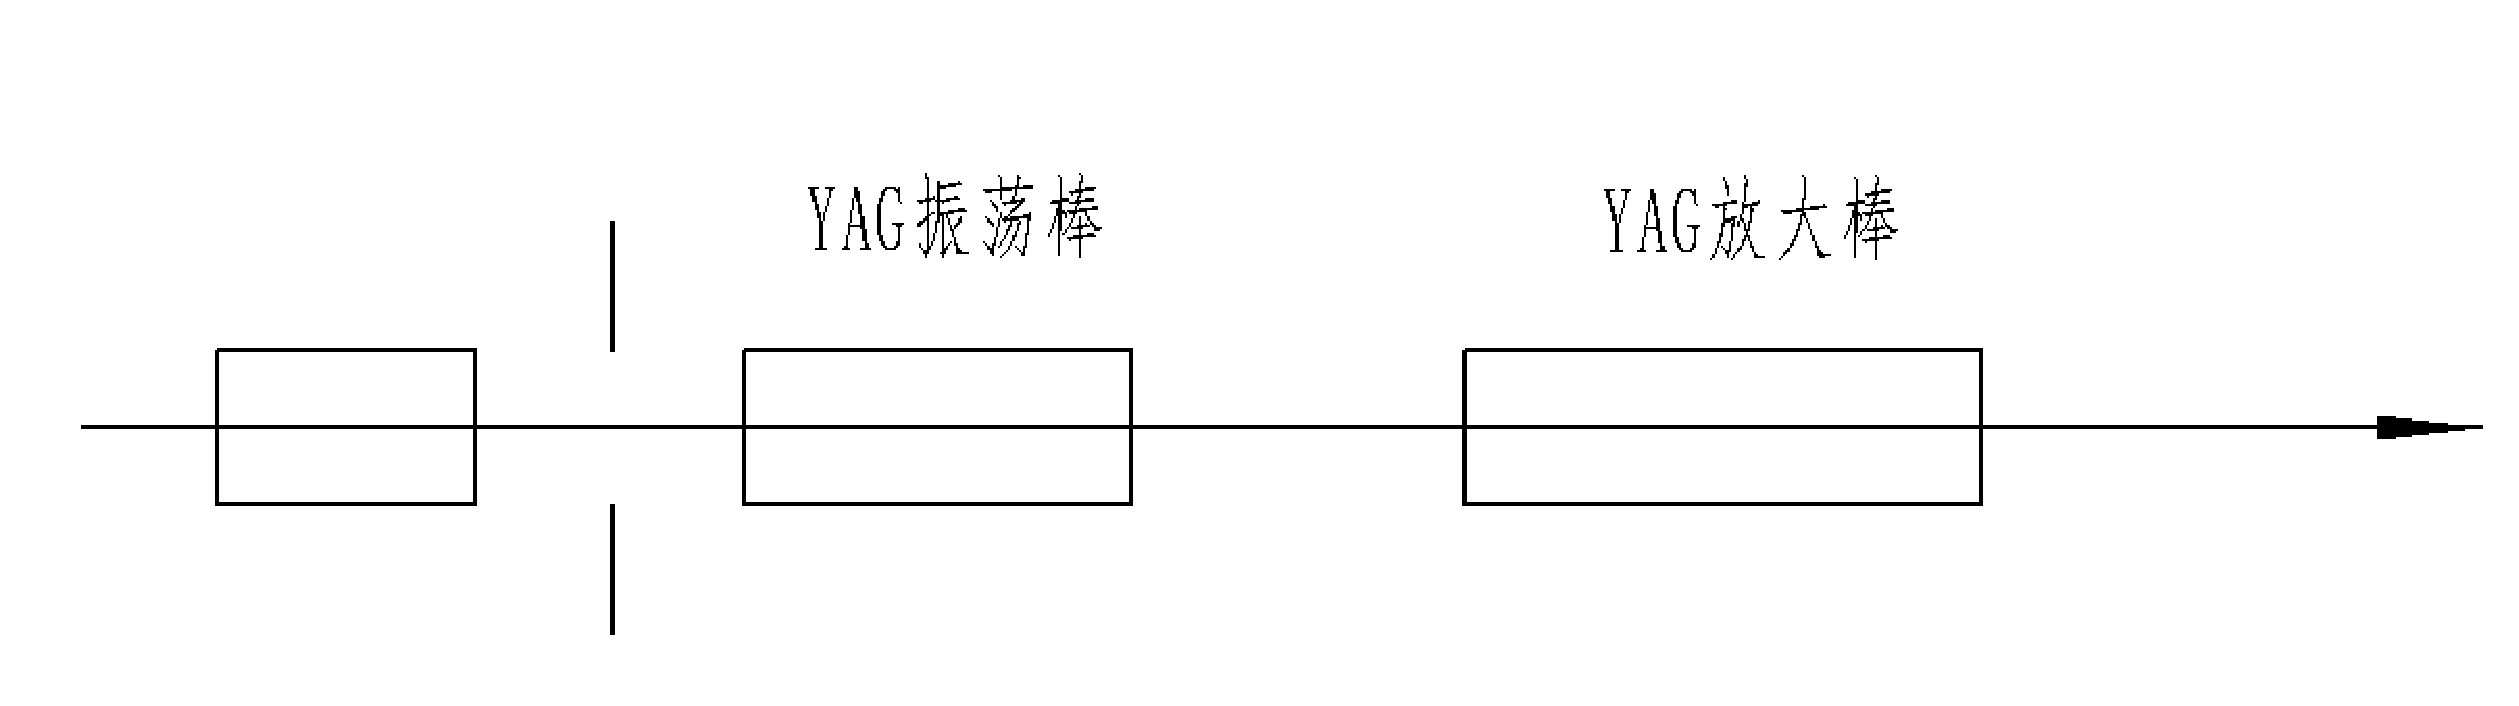
\includegraphics[width=13cm,height=3cm]{1.eps}
			\figcaption{第一次调整激光光路}\label{1.eps}
		\end{center}
		\item 放入输出镜$M_{2}$,调整$M_{2}$,使其反射光沿着原路返回至小孔。
		\item 放入全反镜$M_{1}$,调整$M_{1}$,使其反射光沿着原路返回至小孔,如图3所示。
		\begin{center}
				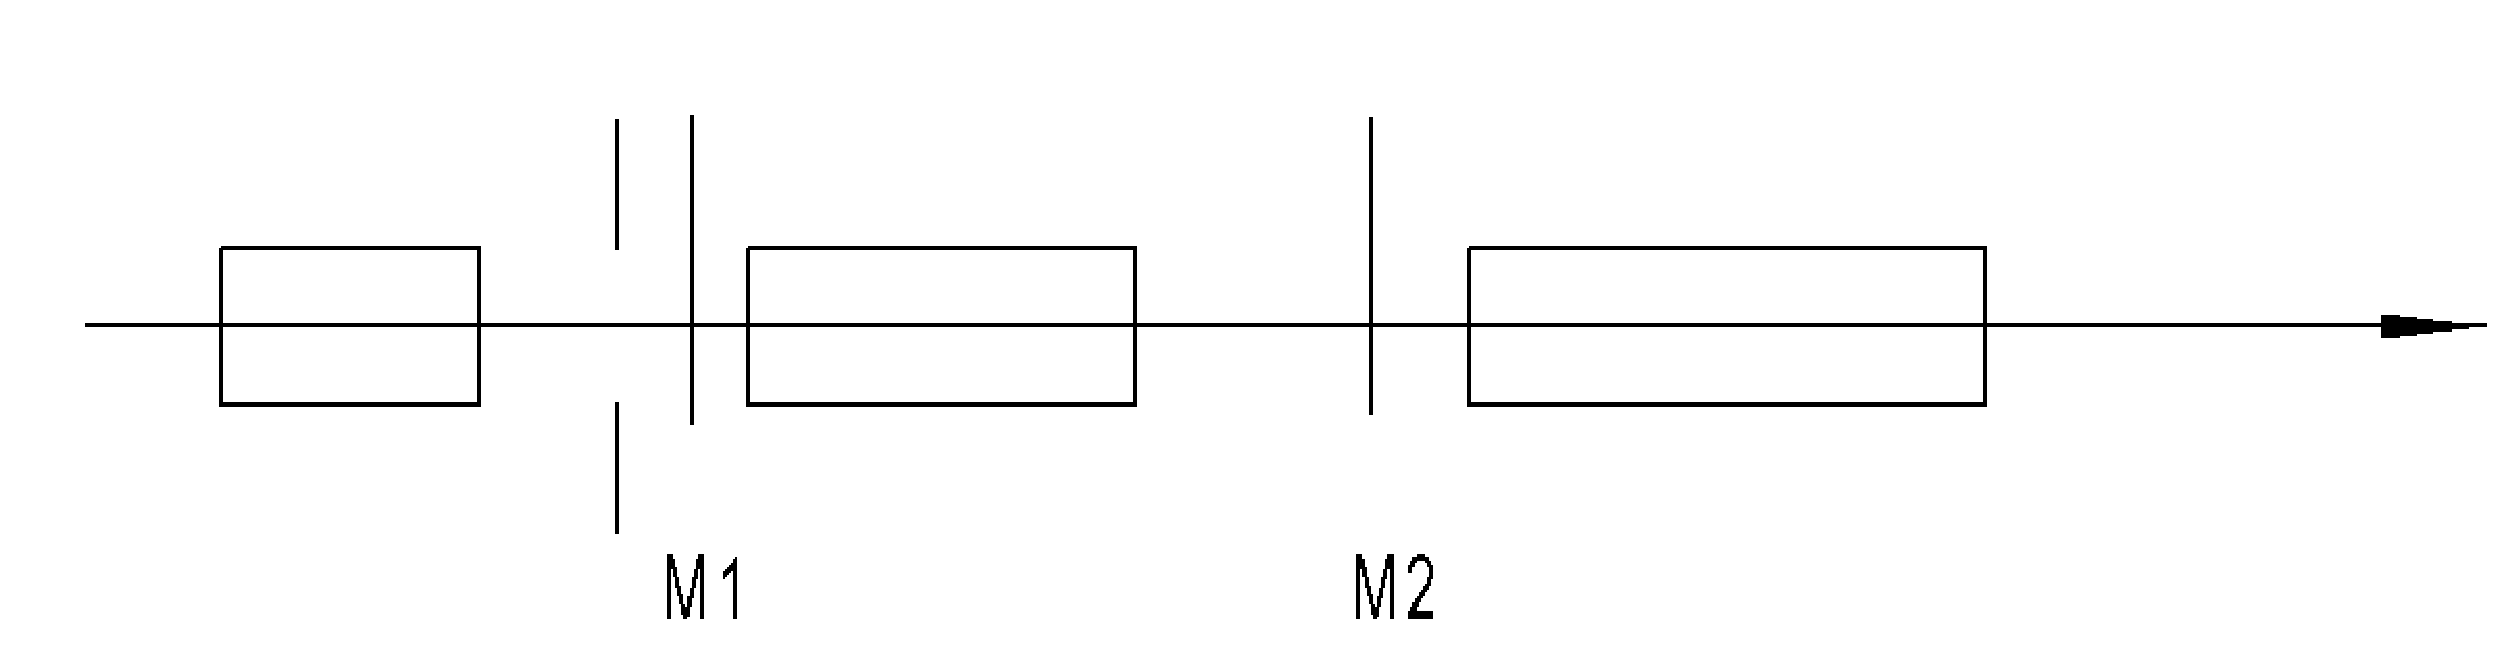
\includegraphics[width=13cm,height=3cm]{2.eps}
				\figcaption{第二次调整光路}\label{2.eps}
		\end{center}
	\end{enumerate}
\item 接通电源,调整出振荡器激光
	\begin{enumerate}
		\item 开启激光电源开关,冷却水泵启动;
		\item 按下预燃(Simmer)按钮,泵浦氙灯点亮;
		\item 按下振荡器电源工作按钮,调节泵浦电压,仔细反复调整反射镜$M_{1}$,$M_{2}$,使其激光振荡器能输出稳定、均匀的激光
	\end{enumerate}
\item 调整出放大器激光
	
	按下放大器电源工作按钮,调节泵浦电压,在调整出振荡器激光后,仔细调整放大器,使其振荡器激光能够全部通过激光放大器,得到整个激光装置的激光输出,其激光光斑是个上下左右都对称的均匀圆形光斑。
\end{enumerate}
\subsection{实验数据}
	\begin{enumerate}
		\item 按照图4光路排布,将示波器接入打印机,输出其自由振荡激光波形。分析其波形形成原理。
		\begin{center}
		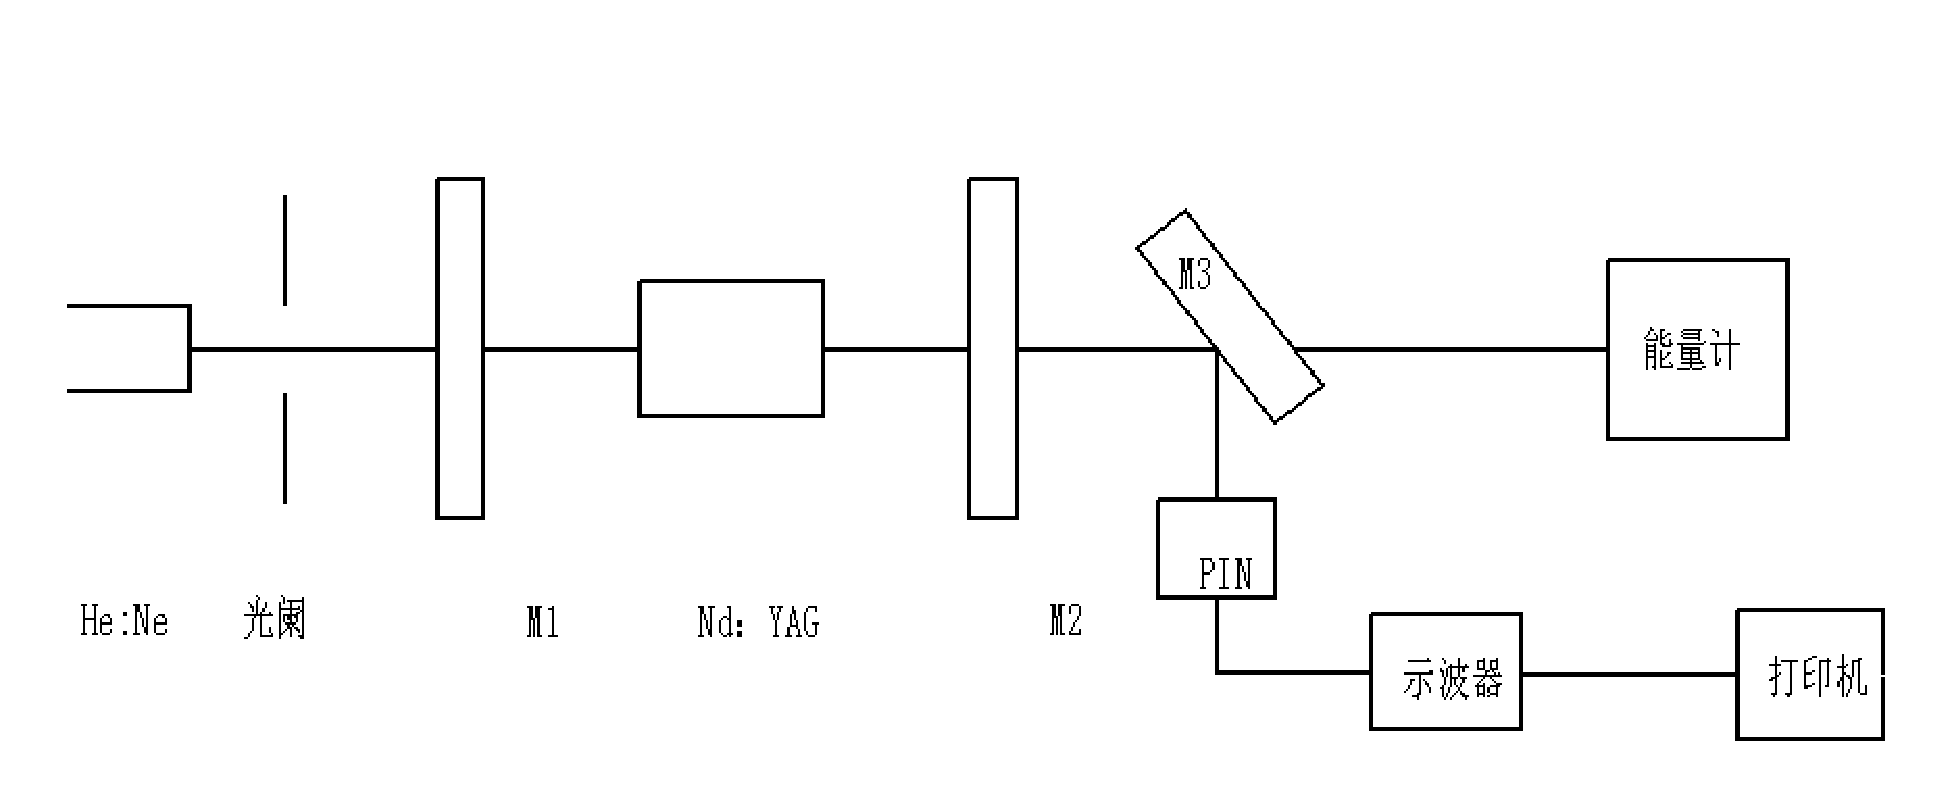
\includegraphics[width=15cm,height=4.5cm]{3.eps}
		\figcaption{光路排布}\label{3.eps}
		\end{center}
		\item 将透镜放在激光放大器后,仔细调整透镜方向,测量出透镜焦距,把实验卡片夹在靶架上,测量好时机焦距
		\item 同时打开激光振荡器和激光放大器,调整适合的泵浦电压,使其高功率激光作用在实验卡片上,卡片上会出现一个针眼大的小孔。
	\end{enumerate}
测量得到的实验数据如下:
\begin{center}
	\tabcaption{原始数据记录}
	\begin{tabular}{|c|c|c|c|c|c|}
		\hline
		电压(V)&本底能量(mJ)&本底加激光能量(mJ)&电压(V)&本底能量(mJ)&本底加激光能量(mJ)\\ \hline
		\multirow{3}{*}{放大前}&373&480&\multirow{3}{*}{750}&408&611\\
		\cline{2-3} \cline{5-6}	
						     &373&455& &409&679\\
		\cline{2-3}	\cline{5-6}
							 &382&462& &409&634\\	\hline
		\multirow{3}{*}{0}	 &402&467&\multirow{3}{*}{800}&406&627\\
		\cline{2-3} \cline{5-6}
							 &423&506& &421&751\\
		\cline{2-3} \cline{5-6}
							 &416&470& &412&761\\ \hline
		\multirow{3}{*}{650} &411&577&\multirow{3}{*}{850}&410&761\\ 
		\cline{2-3} \cline{5-6}
							 &412&567& &396&753\\
		\cline{2-3} \cline{5-6}
						   	 &412&576& &405&794\\ \hline
		\multirow{3}{*}{700} &411&599&\multirow{3}{*}{900}&400&880\\
		\cline{2-3} \cline{5-6}
							 &410&557& &392&870\\
		\cline{2-3} \cline{5-6}
							 &414&591& &394&954\\ \hline
	\end{tabular}
\end{center}
	

\section{实验注意事项}
	\begin{enumerate}
\item 不要用眼睛直射准直光源$He-Ne$光;
\item 开启激光电源钱,戴上激光防护镜;
\item 泵浦氙灯易破碎,不要碰及。
	\end{enumerate}

\section{实验数据处理}
\subsection{实验数据处理方法}
\begin{enumerate}
	\item 求出激光能量
	\begin{equation}
		E_{\mbox{\fontsize{6}{0}激光}}=E_{\mbox{\fontsize{6}{0}本底+激光}}-E_{\mbox{\fontsize{6}{0}本底}}
	\end{equation}
	\begin{equation}
		E_{mean}=\frac{\sum_{1}^{3} E_{i}}{3}
	\end{equation}
\item 计算功率的放大倍数
\begin{equation}
	G_{p}=\frac{I_{\mbox{\fontsize{6}{0}放}}}{I_{\mbox{\fontsize{6}{0}振}}}=G_{e}
\end{equation}

\item 		
以$E_{mean}$为纵坐标,电压U为横坐标,作拟合曲线,如图5所示,之后我们发现由于实验过程中测量误差的存在,直线的拟合情况并不是很好,所以我们设计去除实验中的一些误差较大的点再进行绘图,如图6所示,我们选择了存在的数和平均数的差值作为判断依据,如果大于某一个数,就将其舍去,再进行直线拟合,发现确实由于实验的误差存在,误差取小之后直线的拟合后的参数也反应的比之前的好。
\end{enumerate}
\subsection{实验处理结果}
\begin{center}
	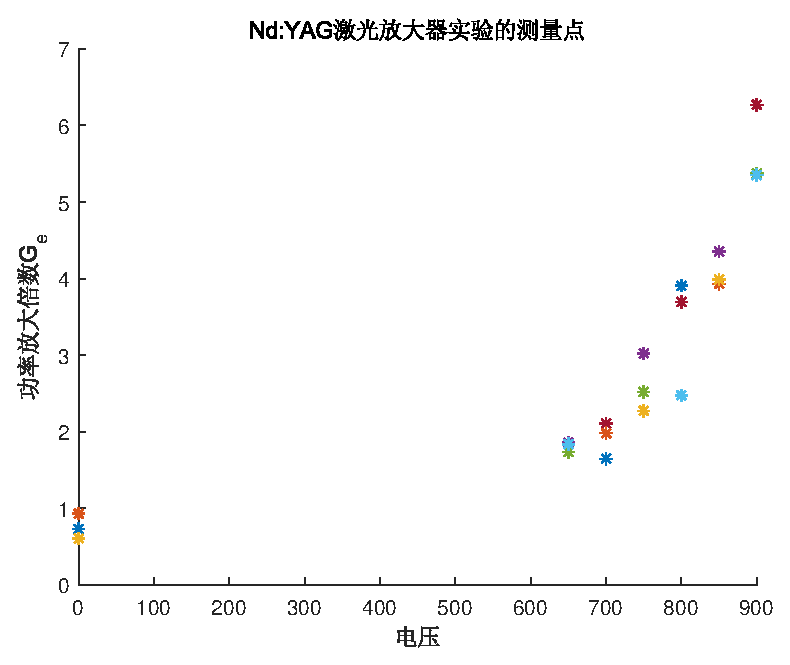
\includegraphics[height=10cm]{Nd_AllPoints.eps}
	\figcaption{数据点绘制}\label{AllPo}
\end{center}
\begin{center}
	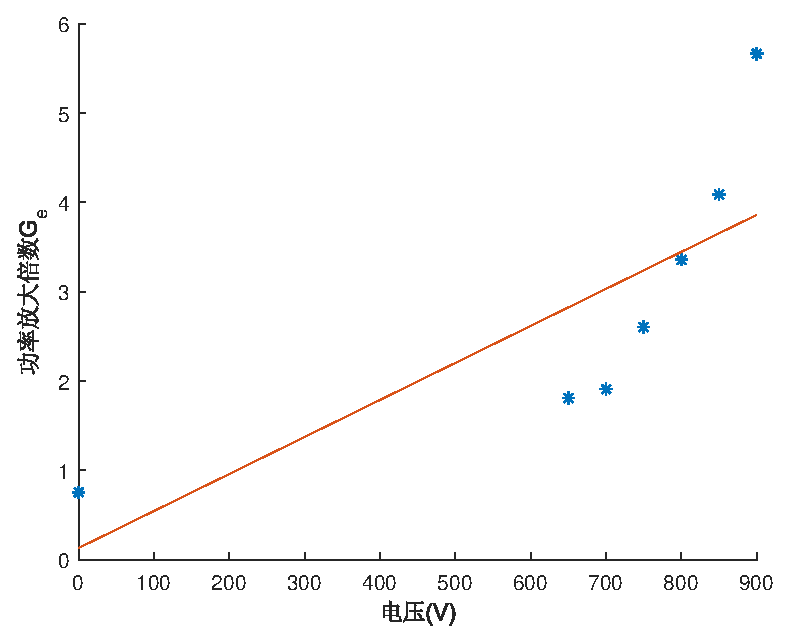
\includegraphics{Nd_AllFitCurve.eps}
	\figcaption{取平均再拟合}\label{fitall}
\end{center}

\begin{center}
	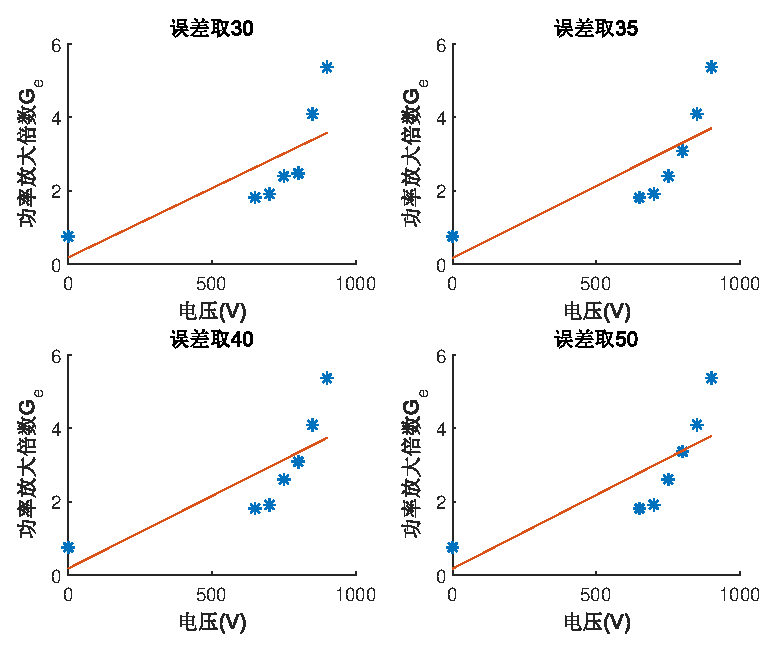
\includegraphics{Nd_DiffErr.eps}
	\figcaption{不同误差范围再拟合}\label{fitdiff}
\end{center}
	\subsection{实验结果分析}	
可以看到,实验得到的点的线性程度并不是很高,只是在大致上看起来呈线性关系,我们分析了如下原因:
\begin{enumerate}
	\item 热电偶测量时候的误差,在等待热电偶冷却至与环境的温度平衡的过程中,我们的用时并没有花费很多,这也就是说,很有可能在未平衡时候就进行测量,下次测量也会在本底上产生误差;
	\item 档纸的拿出和插入时候的误差,可能由于拿出插入时间过快,或者在拿出的时候未完全拿出造成一部分的能量的损耗;
	\item 仪器老旧,造成部分误差。
\end{enumerate}
	

	\subsection{实验代码}
实验代码大体上如下,从Excel中导入数据,将其作差,再计算平均值,再根据公式计算功率放大倍数,计算得到之后作图分析,总共绘制三个图,一个是测量得到的所有数据,一个是直接求平均得到的拟合图,一个是限定误差得到的拟合图。
	
主函数如下:
		\lstinputlisting[language={MATLAB},
		numbers=left, numberstyle={\normalsize },	commentstyle=\color{red!50!green!50!blue!50}, 
		frame=shadowbox, rulesepcolor=\color{red!20!green!20!blue!20}]
		{code/exp6.m}
	
mean3函数如下:
		\lstinputlisting[language={MATLAB},
		numbers=left, numberstyle={\normalsize },	commentstyle=\color{red!50!green!50!blue!50}, 
		frame=shadowbox, rulesepcolor=\color{red!20!green!20!blue!20}]
		{code/mean3.m}
errorc函数如下:
		\lstinputlisting[language={MATLAB},
		numbers=left, numberstyle={\normalsize },	commentstyle=\color{red!50!green!50!blue!50}, 
		frame=shadowbox, rulesepcolor=\color{red!20!green!20!blue!20}]
		{code/errorc.m}
plotep6函数如下:
\lstinputlisting[language={MATLAB},
numbers=left, numberstyle={\normalsize },	commentstyle=\color{red!50!green!50!blue!50}, 
frame=shadowbox, rulesepcolor=\color{red!20!green!20!blue!20}]
{code/plotep6.m}
\section{ 思考题与讨论}
	\begin{enumerate}
		\item 由于光学介质有色散,当$He-Ne$光入射时,透镜的焦距$f=16$cm,当激光($\lambda = 1064$nm)入射时,$f=$?
		
		透镜的焦距是其固有属性,所以焦距$f=16c$m。
	
		\item 根据打印的激光自由震荡的波形,分析其尖峰的形成过程
			
 尖峰脉冲形成的原因及过程是脉冲氙灯开始闪光后约0.5ms开始发出激光,一经发光就迅速消耗掉上能级的粒子数,使$\Delta$N降到阈值之下。这样激光发射大约维持1$\mu$m被迫停止。由于闪光灯继续抽运,上能级粒子数迅速积累,$\Delta$N大于阈值后,又再次发射一个激光脉冲,如此继续。所以在氙灯1ms的闪光时间内,输出一系列小的激光尖峰脉冲,每个尖峰脉冲的持续时间约1$\mu$s。
	\end{enumerate}

\end{document}

